\fig{fv:n3:liquid}{旋转液面的切线垂直于局部有效重力}{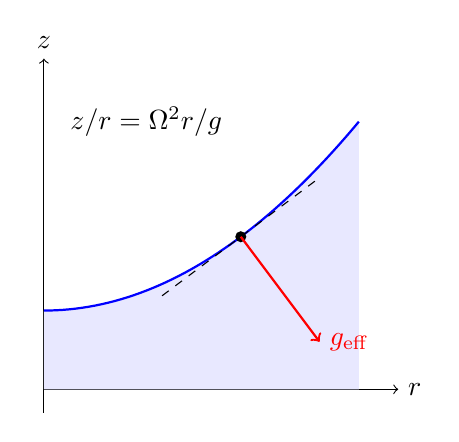
\begin{tikzpicture}[x=1cm,y=1cm]
\draw[->](0,-.3)--(0,4.2)node[above]{$z$};\draw[->](0,0)--(4.5,0)node[right]{$r$};
\fill[blue!9](0,0)--(4,0)--(4,3.4)--plot[domain=4:0,samples=50](\x,{1+.15*\x*\x})--cycle;
\draw[blue,thick,domain=0:4,samples=50]plot(\x,{1+.15*\x*\x});
\fill(2.5,1.9375)circle(2pt);\draw[->,red,thick](2.5,1.9375)--(3.5,.604)node[right]{$\bm g_{\rm eff}$};
\draw[dashed](1.5,1.1875)--(3.5,2.6875);\node at(1.3,3.4){$\dd z/\dd r=\Omega^2r/g$};\end{tikzpicture}}
图\ref{fv:n3:liquid}中液体随容器稳定转动，在转动系相对静止。局部有效重力由向下的 $g$和向外的 $\Omega^2r$合成；自由表面压强处处相同，沿面不能有压强梯度，因此表面必须垂直该合矢量。于是 $g\dd z=\Omega^2r\dd r$。以轴心液面 $(0,z_0)$ 为起点，沿表面积分：
\[
g\int_{z_0}^{z}\dd\zeta=\Omega^2\int_0^r s\,\dd s,
\qquad g[\zeta]_{z_0}^{z}=\Omega^2[s^2/2]_0^r.
\]
这给出 $g(z-z_0)=\Omega^2r^2/2$，与前面的压强法得到同一抛物面。常数 $z_0$还须由总体积确定，不能把原液面高度直接当作旋转后的轴心高度。
